\section{Evaluation of Existing Methods}
\subsection{Baseline Considerations}
It is important to remember that there is no need to 
reinvent the wheel. Since \textit{CodeMirage} has already 
conducted tests on several detection methods, it is 
reasonable to start from their results for the initial 
considerations.

\begin{figure}[H]
    \centering
    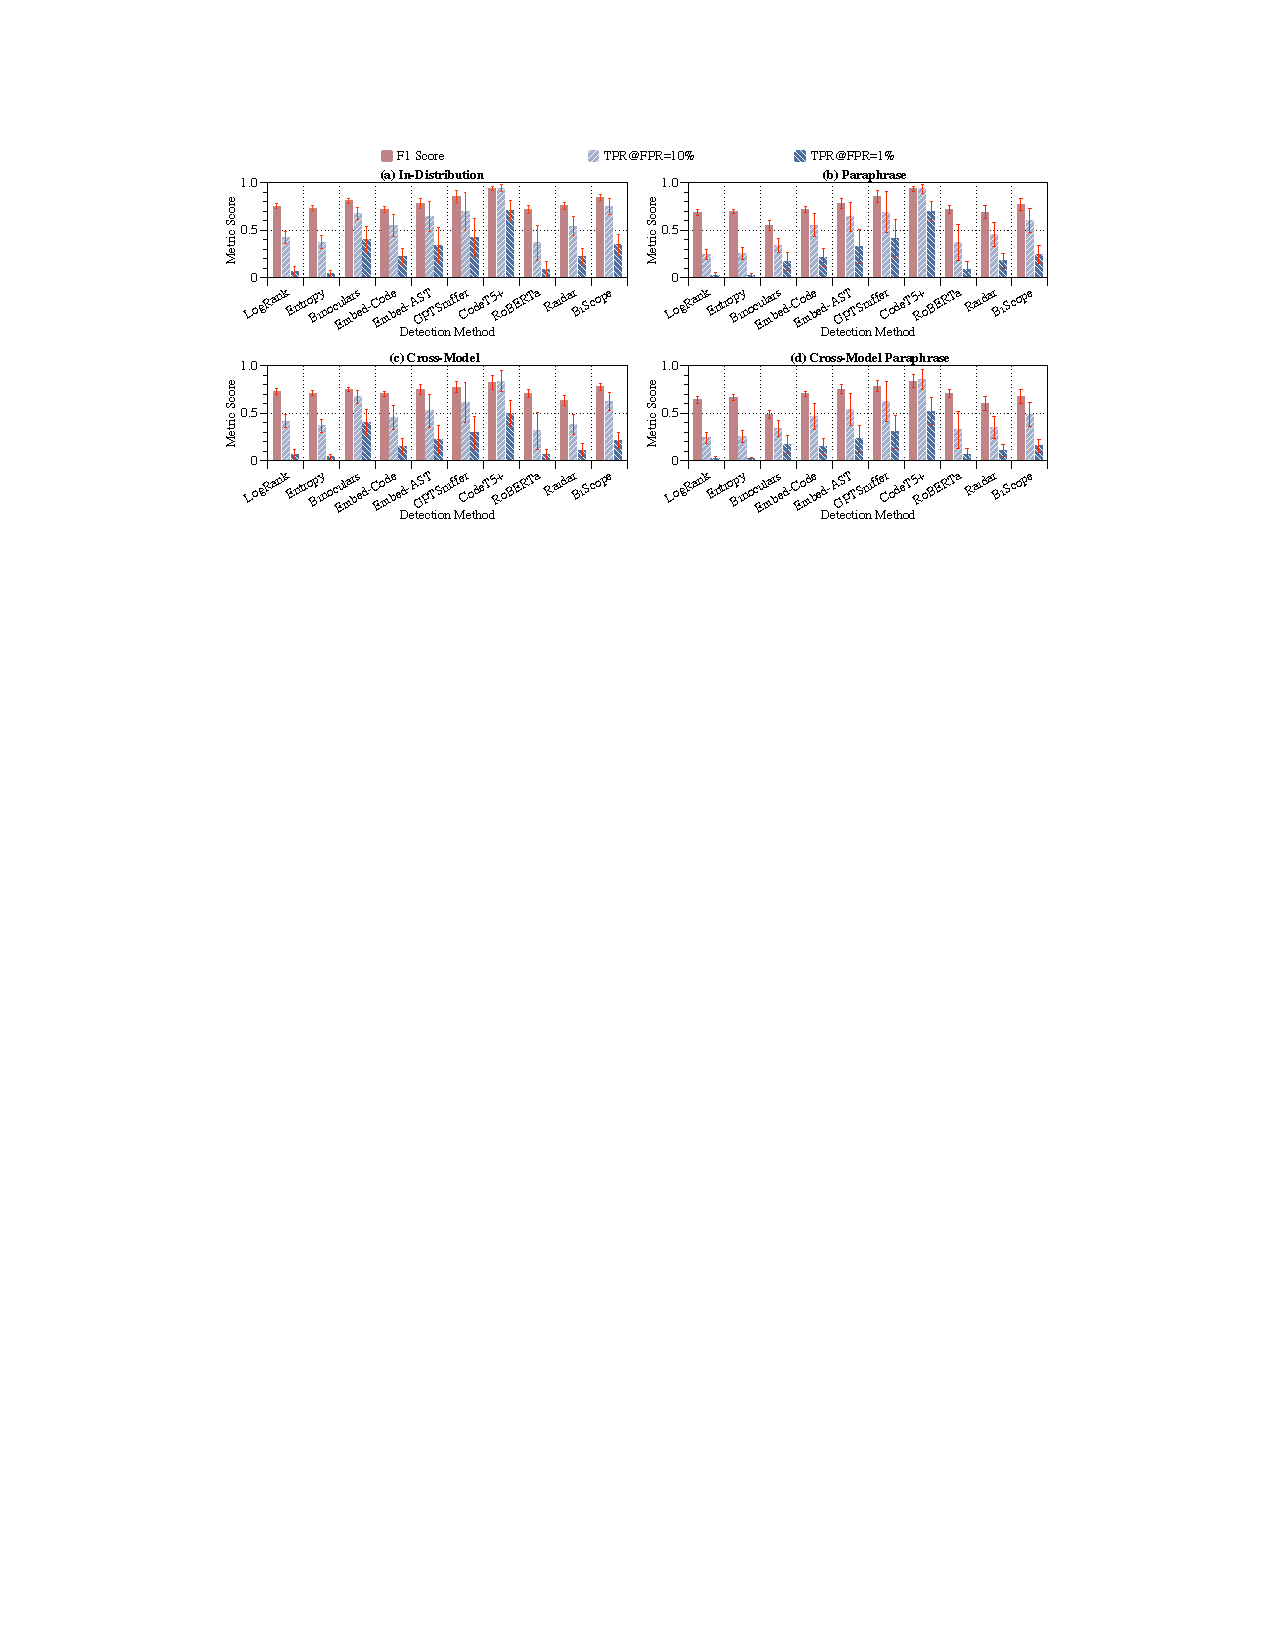
\includegraphics[width=1\textwidth]{img/tests/CodeMirage-tests.pdf}
    \caption{CodeMirage's tests}
    \label{fig:CodeMirage-tests}
\end{figure}

CodeMirage evaluates 10 detection methods, which are divided into four categories:
\begin{enumerate}
    \item \textbf{Zero-shot detectors}: \textit{logRank}, \textit{entropy}, \textit{binoculars}.\\
    These are methods based on the computation of code-related metrics and do not require any training.
    
    \item \textbf{Embedding-based detectors}: \textit{codeXEmbed-2B}.\\
    These methods use LLMs that are not fine-tuned for classification, coupled with lightweight classifiers.
    
    \item \textbf{Fine-tuned detectors}: \textit{GPTSniffer}, \textit{CodeT5+}, \textit{RoBERTa}.\\
    These approaches are based on the same principles as embedding-based detectors, but are specifically fine-tuned for the classification task.
    
    \item \textbf{Pretrained LLM with downstream detector}: \textit{Raidar}, \textit{Bioscope}.\\
    These methods leverage metrics that can be extracted from internal LLM values, such as hidden states.
\end{enumerate}

After analyzing the methods divided into these four subcategories, 
the authors of CodeMirage themselves pointed out that fine-tuned 
detectors are the most affected by domain shifts. Indeed, by analyzing 
their plots, it is clear that all evaluation metrics for methods in the 
fine-tuned detectors category significantly drop in a cross-domain context 
(Figure~\textit{CodeMirage-tests}). 

This is easily justified by the fact that fine-tuned methods perform 
very well in in-distribution settings because they learn the 
characteristics of the LLMs that generate the code—almost as if 
they learn the LLMs' coding style. Even though the performance of 
fine-tuned models decreases when shifting domains, they still remain, 
on average, more effective than methods in the other categories.

Nonetheless, an important clarification is needed: all the code samples 
in the dataset actually belong to the same “category.” As noted by several 
works proposing code detectors, the context in which code is written is a 
non-negligible factor. Since all the samples in the dataset come from 
GitHub-style sources (i.e., open-source projects), it is reasonable to 
expect that fine-tuned models applied to code from different contexts 
(such as competitive programming) would perform significantly worse.

The most important insight that CodeMirage provides is that, if the 
goal is to detect LLM-generated code from a known group of models 
within a specific coding domain, fine-tuning a model specifically for 
classification is the most effective method.

That said, it is far more interesting to have a detection method that 
is easy to use and does not require specific training for each 
application domain. By analysing the zero-shot methods, we 
immediately observe that their performance at TPR@FDR=1\% is 
extremely low, with the notable exception of \textit{binoculars}, 
which achieves results comparable to those of fine-tuned methods. 
This offers hope for zero-shot methods to reach good performance 
while maintaining potentially unlimited applicability across domains.


\subsection{Test framework}
